\chapter{Описание принципа работы подсистемы питания}
\section{Описание схемотехнического решения}
\subsection{PoE-контроллер}
\hspace{1cm} 
Подсистема питания состоит из двух частей:

\begin{enumerate}
    \item Микросхема контроллера PoE TPS2376 с обвязкой
    \item DC-DC преобразователь LMR36520FADDA с обвязкой 
\end{enumerate}

За основу схемотехнического решения контроллера PoE взята типичная применяемая схема для
микросхемы TPS2376, которая была доработана и изображена на рисунке \ref{ris:311}.

\begin{figure}[H]
    \centering
    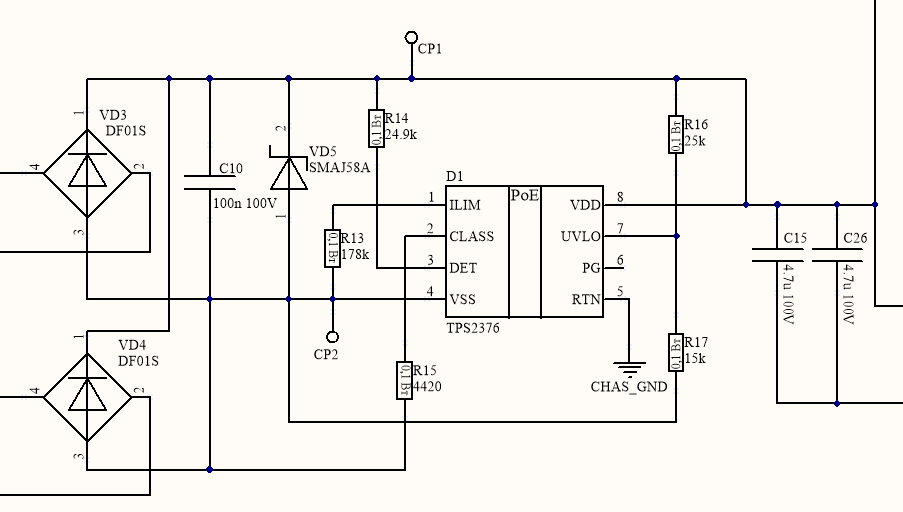
\includegraphics[scale = 0.6]{ris311.png}
    \caption{Принципиальная электрическая схема обвзяки TPS2376 }
    \label{ris:311}
\end{figure}

На четвертый контакт диодного моста VD3 приходит сигнал с четвертого и пятого контактов 
Ethernet-разъема RJ45, которые отвечают за подключение отрицательного напряжения PoE.
На второй контакт диодного моста VD3 приходит сигнал с седьмого и восьмого контактов 
Ethernet-разъема RJ45, которые отвечают за подключение положительного напряжения PoE.  
На второй и четвертый контакты диодного моста VD4 приходят сигналы со средней точки согласующего
Ethernet-трансформатора с линий передачи и приема данных. Диодные мосты выпрямляют приходящее
на них переменное напряженине, превращая его в почти постояное с небольшими пульсациями.

Керамический конденсатор C10 является фильтрующим по питанию. Фильтрующие конденсаторы предназначены 
для фильтрации питания микросхем от высокочастотных помех и обычно их номинал равень 100 нФ.
Такие конденсаторы встречаются довольно  часто, и в дальнейшем в этой дипломной работе не будет 
описываться их назначение. Так как максимальное напряжение PoE 57 В, то рабочее напряжение 
конденсатор C10 выбрано почти с двойным запасом для повышения срока службы и надежности схемы.

Супрессор VD5 предназначен для защиты микросхемы от перенапряжения, например в случае поражения
линии статикой и расчитан на рабочее напряжение в 58 В. 

Резистор R13 предназначен для ограничения пускового тока. Ограничение пускового тока ограничивает
протекание тока через выходные конденсаторы C15 и С16 в начальный момент их зарядки и не дает 
вызвать просадку напряжения ниже, чем задает делитель напряжения R16, R17 на выводе UVLO.  

Обычно сопротивление резистора R14 должно быть равно 24,9 кОм. Rdet подключен к входной линии, 
когда VDD находится в диапазоне от 1,4 В до 11,3 В, и отключается,
когда напряжение на линии выходит за пределы этого диапазона, чтобы сэкономить энергию.
Этот диапазон напряжений был выбран для того, чтобы обеспечить возможность обнаружения с 
помощью двух кремниевых выпрямителей между контроллером PoE и разъемом RJ-45.

Значение резистора R15 было выбрано равным 4420 Ом исходя из 
необходимой выходной мощности по таблице \ref{ClassTPS2376}.

\begin{table}[H]
    \caption{Классификация TPS2376} 
    \label{ClassTPS2376}
    \begin{center}
    \begin{tabular}{|c|c|c|c|}
    \hline
    Class & PD POWER, W  &  Rclass, Ohm   & 802.3af LIMITS, mA \\ \hline
    0 & 0,44 -- 12,95  & 4420 &0 -- 4  \\ \hline
    1 & 0,44 -- 3,84 & 953 & 9 -- 12   \\ \hline
    2 & 3,84 -- 6,49 & 549 & 17 -- 20  \\ \hline
    3 & 6,49 -- 12,95 & 357 & 26 -- 30   \\ \hline
    \end{tabular}
    \end{center}
\end{table} 

Вывод VSS подключается к минусу выходного с диодных мостов напряжения, 
а вывод VDD подключается к плюсу этого напряжения.

Вывод PG предназначен для передачи разрешающего сигнала на работу последующих микросхем,
в данной схеме нет потребности в реализации дополнительных условий или задержек включения
дальнейших элементов схемы, поэтому он не используется.

Вывод UVLO используется с внешним резисторным делителем между VDD и VSS для установки 
верхнего и нижнего порогов UVLO. TPS2376 включает выход, когда напряжение UVLO превышает верхний 
порог UVLO. Когда начинает течь ток, VDD проседает из-за сопротивления кабеля и динамического 
сопротивления входных диодов. Нижний порог UVLO должен быть ниже самого низкого напряжения, 
которого достигает вход. Коэффициент делителя должен быть выбран таким образом, 
чтобы получить примерно 2,5 В на выводе UVLO, когда VDD находится на требуемом 
напряжении включения. Поэтому R16 и R17 выбраны номиналом 25 кОм и 1,5 кОм соответственно,
для обеспечения коэффициента деления 16,(6).

Выходные конденсаторы С15 и С26 предназначены для фильтрации выходного напряжения, но взяты 
несколько меньше по номиналу рекомендуемых для уменьшения габаритов устройства. Их рабочее
напряжение так же взято с почти двойным запасом \cite{TPS2376:datasheet}.

Общий принцип работы этого в обеспечении стандрата IEEE 802.3af, который определяет 
процесс безопасного питания по PoE по Ethernet-кабелю и последующего отключения питания, 
если нагрузка отсоединена. Процесс проходит через три рабочих состояния: обнаружение, 
классификация и работа. Смысл процесса заключается в том, что когда нагрузка не подключена,
контроллер PoE периодически проверяет наличие подключенного устройства -- это называется 
обнаружением. Если подключается нагрузка, то контроллер может запросить информацию о том,
сколько энергии она потребует -- это этап классификации. Знание потребности в мощности нагрузки 
позволяет контроллеру PoE разумно отдавать и распределять энергую, в случае нескольких нагрузок,
а так же защищать себя от перегрузки. После этапа классификации контроллер подает питание на 
нагрузку и контролирует линию питания на предмет перегрузки. Если после этого отключить нагрузку,
контроллер снова войдет в исходное состояние обнаружения. Рисунок \ref{ris:312}  илюстрирует 
вышеописанный паттерн поведения контроллера PoE \cite{TPS2376:datasheet}.

\begin{figure}[H]
    \centering
    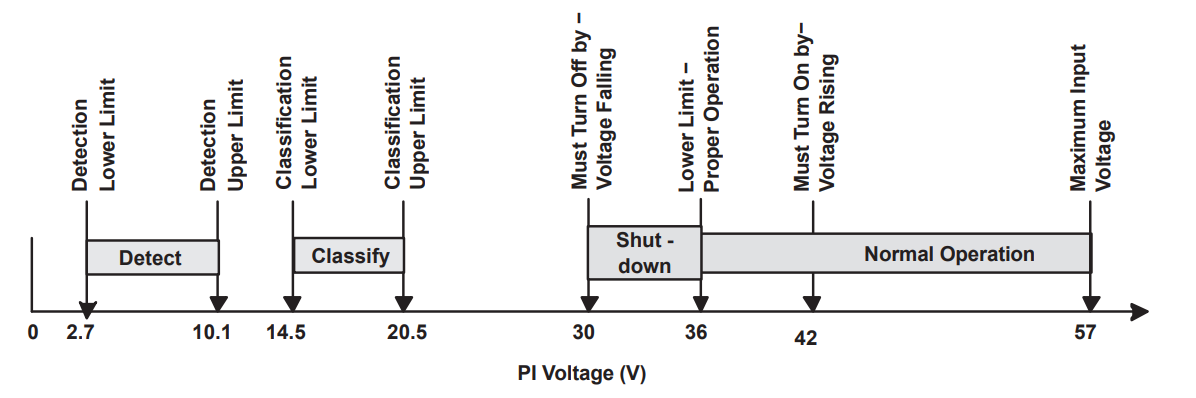
\includegraphics[scale = 0.55]{ris312.png}
    \caption{IEEE 802.3 PD Limits}
    \label{ris:312}
\end{figure}

Ожидаемые осциллограммы в основных узлах этой части схемы представлены на рисунке 
\ref{ris:313} \cite{TPS2376:datasheet}.

\begin{figure}[H]
    \centering
    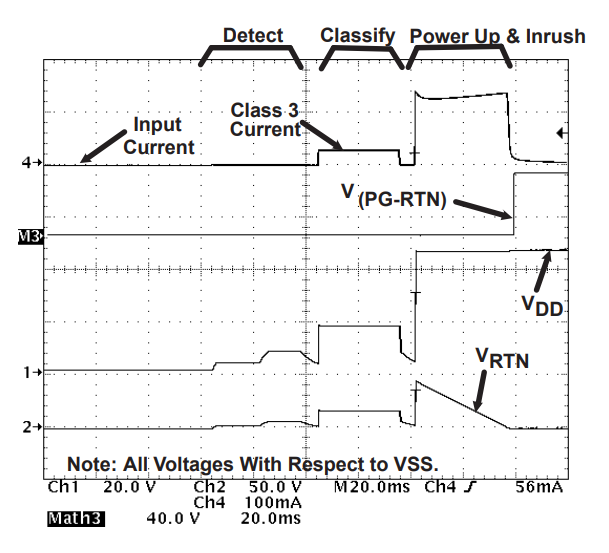
\includegraphics[scale = 0.75]{ris313.png}
    \caption{Осциллограммы TPS2376 при включении}
    \label{ris:313}
\end{figure}

\subsection{DC-DC преобразователь}
\hspace{1cm} 

В качестве изолированного FlyBack-преобразователя было выбрано решение на базе микросхемы LMR36520 
от компании Texas Instruments из-за наличия подробной документации по расчету каждого элемента
обвязки. 

Схемотехническое решение представлено на рисунке \ref{ris:321}.

\begin{figure}[H]
    \centering
    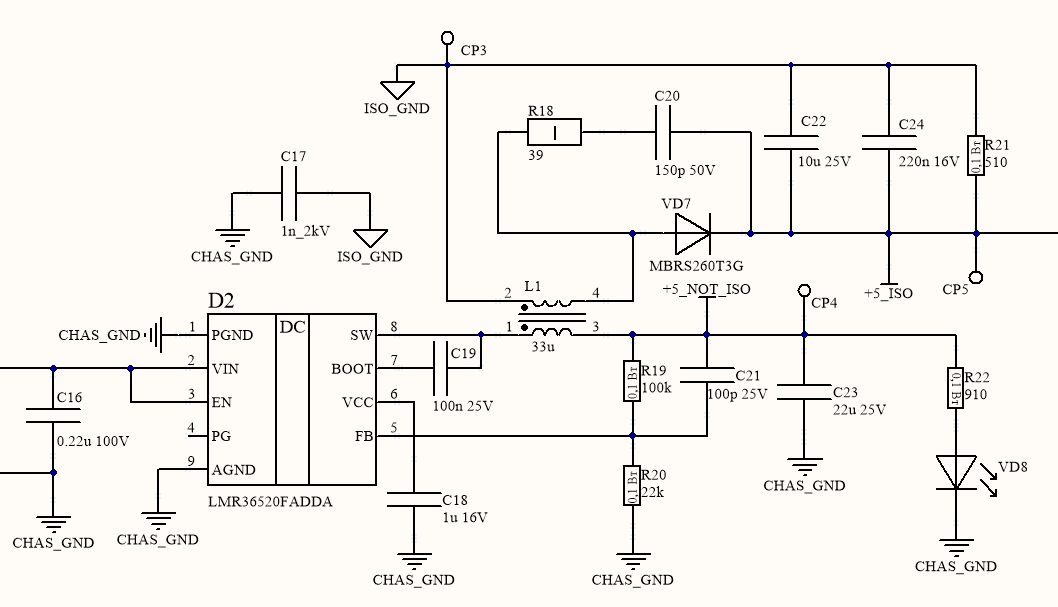
\includegraphics[scale = 0.65]{ris321.png}
    \caption{Принципиальная электрическая схема обвязки LMR36520}
    \label{ris:321}
\end{figure}

Конденсатор С16 является фильтрующим по входному питанию.На вывод VIN приходит напряжение
с выхода PoE-контроллера. Сигнал EN является разрешающим работу преобразователя. Так как
в данной схеме нет потребности в реализации дополнительных условий или задержек включения
DC-DC преобразователя, то этот вывод останется неподключеным. PGND и AGND соединены внутри 
микросхемы и подключаются к <<аналоговой>> земле. 

PG -- это выход флага состояния питания преобразователя, является выходом с открытым стоком. 
В данной схеме нет потребности в отслеживании включения преобразователя, поэтому этот вывод не 
используется. 

FB -- вход обратной связи регулятора, подключается к средней точки резистивного делителя
напряжения.

Вывод VCC является выходом внутреннего стабилизатора на 5 В, в схеме не используется, но подключим
рекомендуемый конденсатор, для возможной потребности при отладке устройства.

К выводу BOOT подключается bootstrap конденсатор, он же конденсатор запуска, номиналом 100 нФ 
\cite{LMR36520:datasheet}. 

Индуктивность L1 выполняет роль накопителя энергии в FlyBack-преобразователях.
Для описания их работы рассмотрим схему замещения, изображенную на рисунке \ref{ris:322}.

\begin{figure}[H]
    \centering
    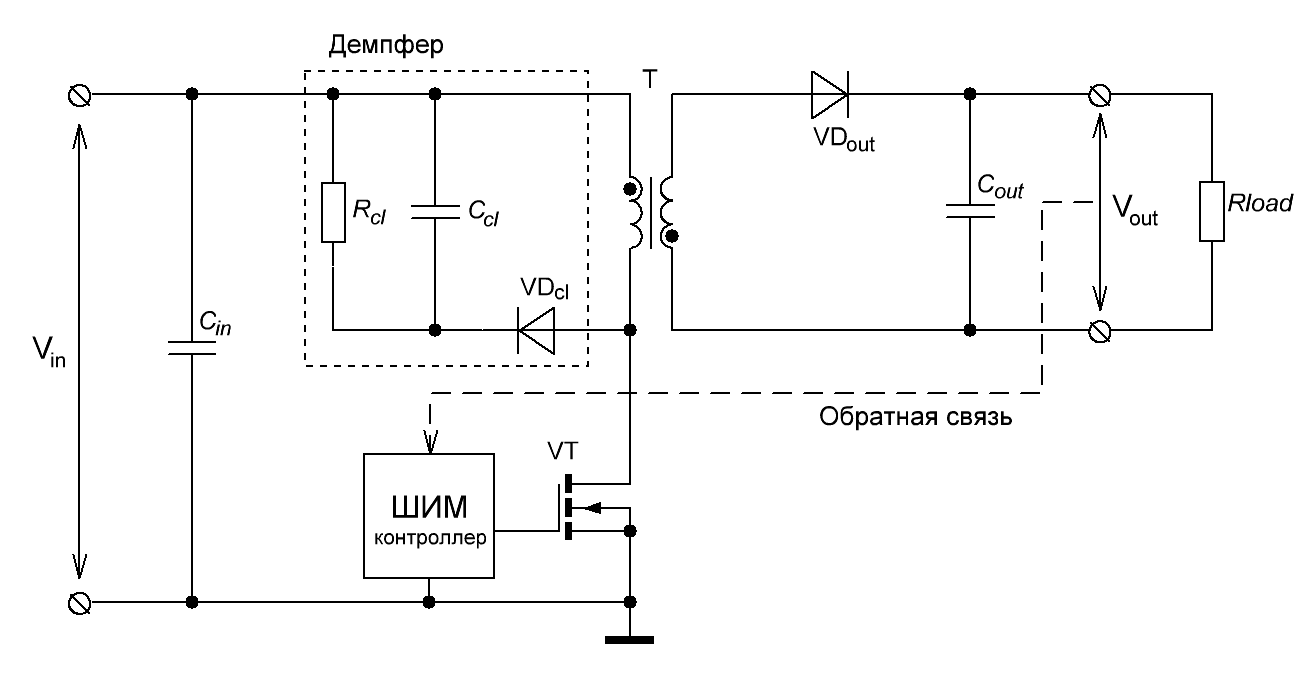
\includegraphics[scale = 0.5]{ris322.png}
    \caption{Упрощенная электрическая схема обратноходового преобразователя}
    \label{ris:322}
\end{figure}

Принцип работы обратноходового преобразователя состоит в следующем. Ключевой транзистор, 
управляемый ШИМ-контроллером, которые в рамках нашего схемотехнического решения встроены
в микросхему LMR36520, коммутирует первичную обмотку трансформатора к источнику питания.
Первичная обмотка обратноходового трансформатора фактически представляет собой дроссель, 
поэтому после коммутации ток через неё линейно растет и энергия накапливается в магнитопроводе. 
К выходному диоду приложено запирающее напряжение и ток во вторичной обмотке не протекает. 
В момент, когда транзистор закрывается, полярность на обмотках в соответствии с законом 
самоиндукции изменяется на противоположную. Диод открывается, ток начинает протекать через
вторичную обмотку трансформатора, и энергия, запасенная в магнитопроводе, переходит в нагрузку. 
И это при закрытом ключе. Далее процесс повторяется. Выходной конденсатор фильтра является 
энергетическим буфером, поддерживающем ток в нагрузке в моменты паузы.
В основе работы преобразователя лежит накопление энергии в индуктивности первичной обмотки 
на первой во времени стадии заряда и передача запасенной энергии на последующей стадии 
передачи энергии. Поскольку стадии накопления и передачи энергии разделены во времени, 
то трансформатор в обратноходовом преобразователе фактически представляет собой индуктивностью 
с двумя или более обмотками. Этот факт Мы используем для уменьшения габаритов схемы и ее упрощения,
заменив трансформатор в нашем преобразователе на две взаимосвязанные катушки индуктивности в 
одном корпусе -- L1, образуя трансформатор с коэффициентом трансформации равным единице
\cite{PowerElectronic:FlyBack} 
\cite{Würth Elektronik:Application Note}
\cite{DC-DC_Book:Recom}.

Вернемся к рассмотрению рисунка \ref{ris:321}. В качестве выходных конденсаторов используются
С23 для неизолированного выхода и С22, С24 для изолированного выхода. В качестве демпферной цепи 
выступают R18, C20 и VD7. Светодиод VD8 и его токоограничительный резистор R22 служат для 
индикации питания. Конденсатор C17 используется для защиты от статики в случае прикосновения ко 
входному разему RJ-45, образуя емкостной делитель с прикоснувшимся человеком, снижая амплитуду 
выброса статического напряжения. 



\section{Расчет элементов схемы}
\hspace{1cm} 

\section{Результаты тестирования}
\hspace{1cm} 